\documentclass{article}

\usepackage[T1]{fontenc} % Umożliwia korzystanie z fontów o kodowaniu T1, które obsługują znaki specjalne używane w językach europejskich.
\usepackage[polish]{babel} % Dostosowuje formatowanie dokumentu do zasad języka polskiego (np. łamanie wierszy, tytuły sekcji).
\usepackage[utf8]{inputenc} % Umożliwia korzystanie z kodowania UTF-8, które obsługuje znaki specjalne i diakrytyczne.
\usepackage{graphicx} % Umożliwia wstawianie obrazów do dokumentu.
\usepackage{subcaption} % Umożliwia tworzenie podpisów dla podobrazów.
\usepackage[margin=2cm]{geometry} % Umożliwia dostosowanie marginesów dokumentu.
\usepackage{listings} % Umożliwia wstawianie kodu źródłowego do dokumentu z odpowiednim formatowaniem.
\usepackage{color} % Umożliwia korzystanie z kolorów w dokumencie.
\usepackage{amsmath} % Rozszerza możliwości formatowania równań matematycznych.
\usepackage{xcolor} % Umożliwia tworzenie kolorowych ram dookoła tekstu.
\usepackage{systeme} % Umożliwia tworzenie systemów równań.
\usepackage{indentfirst} % Powoduje, że pierwszy akapit po tytule sekcji jest wcięty.
\usepackage{dsfont} % Umożliwia korzystanie z dodatkowych fontów, np. dla oznaczeń zbiorów liczbowych.
\usepackage{etoolbox} % Pozwala modyfikować pakiety UŻYWAĆ OSTROŻNIE
\usepackage{blindtext} % Pozwala automatycznie pisać blok lorem ipsum
\usepackage{fancyhdr} % Pozwala na stopki u góry i na dole strony
\usepackage{hyperref} % Umożliwia używanie hyperlinków
\usepackage[justification=centering]{caption}
\hypersetup{
  colorlinks = true,
  linkcolor = black,
  urlcolor = blue,
  pdftitle = {Sprawozdanie z Laboratorium 5} 
}
\patchcmd{\section}{\thispagestyle{plain}}{\thispagestyle{fancy}}{}{}

\definecolor{red}{RGB}{245, 63, 60}
\definecolor{blue}{RGB}{59, 69, 245}
\definecolor{green}{RGB}{72, 225, 17}
\definecolor{yellow}{RGB}{245, 207, 59}

\begin{document}
  \pagestyle{fancy} % pozwala korzystać z pakietu fancyhdr
  \fancyhf{} % clear existing header/footer entries
  \fancyfoot[C]{\thepage}
  \renewcommand{\headrulewidth}{0pt} % Usuń linię na górze strony
  \renewcommand{\footrulewidth}{0.4pt} % Dodaj linię na dole strony  
  \addtolength{\footskip}{0cm} % Zmienia pozycję linii w stopce

  \title{Elektronika Cyfrowa \\ {\large Sprawozdanie z Laboratorium 5}}
  \date{15.05.2024}
  \author{Tomasz Dziób\\{\small Grupa 15}}
  \maketitle

  % Ustawienie Spisu treści do paragrafów 
  \setcounter{tocdepth}{4} % Uwzględnij do typu \paragraph in Spisie treści
  \setcounter{secnumdepth}{4} % Numerowanie do typu \paragraph
  \small \tableofcontents
  \pagebreak

  \section{Wstęp teoretyczny}
    \subsection{Przerzutnik JK}
      Przerzutnik typu JK to jeden z podstawowych rodzajów przerzutników synchronicznych bistabilnych. Przerzutnik ma wejścia informacyjne J i K, zegarowe C, wyjście proste Q i jego negację ~Q. Często posiada również asynchroniczne wejścia kasujące R (Reset) i ustawiające S (Set).

      \begin{figure}[!ht]
        \begin{minipage}{.5\textwidth}
            \centering
            \begin{tabular}{|c|c|c|}
            \hline
            \textbf{J} & \textbf{K} & \textbf{Q} \\
            \hline
            0 & 0 & stan się nie zmienia \\
            \hline
            1 & 0 & 0\\
            \hline
            0 & 1 & 0\\
            \hline
            1 & 1 & zmiana stanu na przeciwny\\
            \hline
            \end{tabular}
            \caption{Tablica prawdy dla przerzutnika JK,
            \\Źródło: Opracowanie własne}
        \end{minipage}
        \begin{minipage}{.5\textwidth}
          \centering
          \includegraphics[scale=0.65]{grafiki/JK_Flip-flop.eps}
          \caption{Schemat wejść/wyjść przerzutnika JK,
          \\Źródło: \href{https://pl.wikipedia.org/wiki/Plik:JK_Flip-flop.svg}{Wikipedia}}
        \end{minipage}
      \end{figure}

      Wejścia informacyjne J i K odpowiadają wejściom S i R przerzutnika RS. Przerzutnik JK \underline{nie ma stanów wejściowych niedozwolonych}. W przypadku jednoczesnego podania sygnałów 1 na wejścia J i K, stan przerzutnika zmieni się na przeciwny
      (w chwili wyzwolenia sygnałem zegarowynm) na jego podstawie można zbudować wiele innych rodzajów przerzutników np. typu D.

    \subsection{Przerzutnik D}
      Jeden z podstawowych rodzajów przerzutników synchronicznych. Przerzutnik ten przepisuje stan wejścia informacyjnego D na wyjście Q. Przepisanie informacji następuje tylko przy odpowiednim stanie wejścia zegarowego, dlatego nazywa się go układem opóźniającym.

      \begin{figure}[!ht]
        \begin{minipage}{.5\textwidth}
            \centering
            \begin{tabular}{|c|c|}
            \hline
            \textbf{D} & \textbf{Q} \\
            \hline
            1 & 1 \\
            \hline
            0 & 0 \\
            \hline
            \end{tabular}
            \caption{Tablica prawdy dla przerzutnika D,
            \\Źródło: Opracowanie własne}
        \end{minipage}
        \begin{minipage}{.5\textwidth}
          \centering
          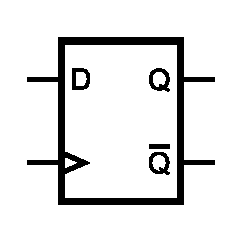
\includegraphics[scale=0.65]{grafiki/D_Flip-flop_(Simple)_Symbol.eps}
          \caption{Schemat wejść/wyjść przerzutnika D,
          \\Źródło: \href{https://pl.wikipedia.org/wiki/Plik:D_Flip-flop_(Simple)_Symbol.svg}{Wikipedia}}
        \end{minipage}
      \end{figure}

      \subsubsection{Wyzwalany zboczem}
        Przerzutnik D może być wyzwalany zboczem, narastającym lub opadającym. Oznacza to, że zmiana stanu przerzutnika następuje w momencie zmiany stanu sygnału zegarowego w określony sposób.

        \begin{enumerate}
          \item \textbf{Zbocze narastające} \\
          Przerzutnik D jest aktywowany w momencie, gdy sygnał zegarowy przechodzi z niskiego stanu (0) do wysokiego stanu (1).

          \item \textbf{Zbocze opadające} \\
          Przerzutnik D jest aktywowany w momencie, gdy sygnał zegarowy przechodzi z wysokiego stanu (1) do niskiego stanu (0).
        \end{enumerate}

        \begin{figure}[!ht]
          \begin{minipage}{.5\textwidth}
            \centering
            \includegraphics[scale=0.25]{grafiki/narastajace.jpg}
            \caption{Przebieg czasowy przerzutnika D wyzwalanego zboczem narastającym,
            \\Źródło: Opracowanie własne}
          \end{minipage}
          \begin{minipage}{.5\textwidth}
            \centering
            \includegraphics[scale=0.25]{grafiki/opadajace.jpg}
            \caption{Przebieg czasowy przerzutnika D wyzwalanego zboczem opadającym,
            \\Źródło: Opracowanie własne}
          \end{minipage}
        \end{figure}

        W chwili tego przejścia w obu przypadkach, przerzutnik przechwytuje wartość sygnału wejściowego D i ustawia wyjście Q na tę wartość.

        \pagebreak

      \subsubsection{Typu \textquotedblleft zatrzask\textquotedblright}
      Drugim typem wyzwalania jest typ \textit{Latch}.
      Gdy sygnał zegarowy na wejściu C jest wysoki (1) -- \textquotedblleft Zatrzask jest otwarty\textquotedblright \mbox{}  i wartość na wejściu D jest przekazywana na wyjście Q. Zatrzask \textquotedblleft przepuszcza\textquotedblright \mbox{}wartość wejściową.
      Natomiast gdy jest niski (0) -- Przysłowiowy zatrzask zamyka się, a wyjście Q zachowuje swoją poprzednią wartość, niezależnie od zmian na wejściu D.

      \begin{figure}[!ht]
          \centering
          \includegraphics[scale=0.25]{grafiki/latch.jpg}
          \caption{Przebieg czasowy przerzutnika D wyzwalany poziomem,
          \\Źródło: Opracowanie własne}
      \end{figure}

    \subsection{Przerzutnik Synchroniczny RS -- latch}
      Jest to wersja przerzutnika RS synchronizowana zegarem który działa na zasadzie poziomów sygnału wejściowego. Jest to przerzutnik zatrzaskowy, co oznacza, że jego stan zależy od poziomu sygnału sterującego, a nie od zbocza sygnału zegarowego. Czyli oznacza to, że układ reaguje na wejścia S i R tylko gdy zegar jest w sa
    \begin{figure}[!ht]
      \centering
      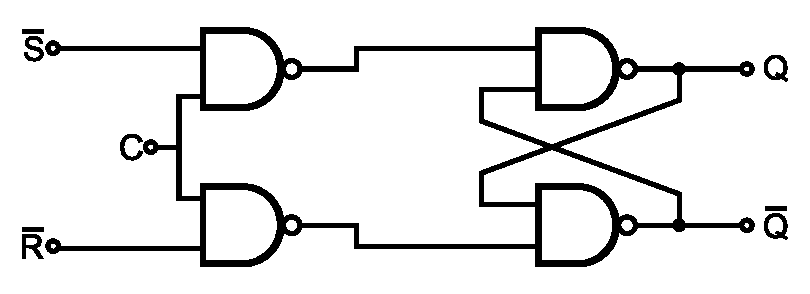
\includegraphics[scale=0.55]{grafiki/SR_NAND_Async_latch.eps}
      \caption{Schemat Przerzutnika asynchronicznego RS typu latch zbudowany z bramek NAND,
      \\Źródło: Opracowanie własne}
    \end{figure}

    \subsection{Liczniki zbudowane przy użyciu przerzutnika JK}
      Licznik -- nazywamy tak układ cyfrowy służący do zliczania impulsów. Na wyjściu licznika pojawia się zakodowana binarnie liczba impulsów podanych na wejście zliczające. Oprócz wejścia impulsów zliczanych, licznik posiada zazwyczaj wejście ustawiające stan początkowy (zerowanie licznika).

      Wyróżniamy rodzaje liczników:
      \begin{enumerate}
        \item  liczące w przód (następnikowe)
        \item  liczące w tył (poprzednikowe)
        \item rewersyjne (możliwość zmiany kierunku zliczania)
      \end{enumerate}
      
      Oraz możemy podzielić je ze względu na tryb synchronizacji:
      \begin{enumerate}
        \item szeregowe (asynchroniczne)
        \item równoległe (synchroniczne)
      \end{enumerate}
      Na zajęciach zajmowaliśmy się licznikami szeregowymi liczącymi w przód.

      Wyjścia liczników mogą służyć jako układy dzielące (redukujące) częstotliwość sygnałów. Im większa ilość wejść użytych, tym większa będzie redukacja względem oryginalnego sygnału.

      \begin{figure}[!ht]
        \centering
        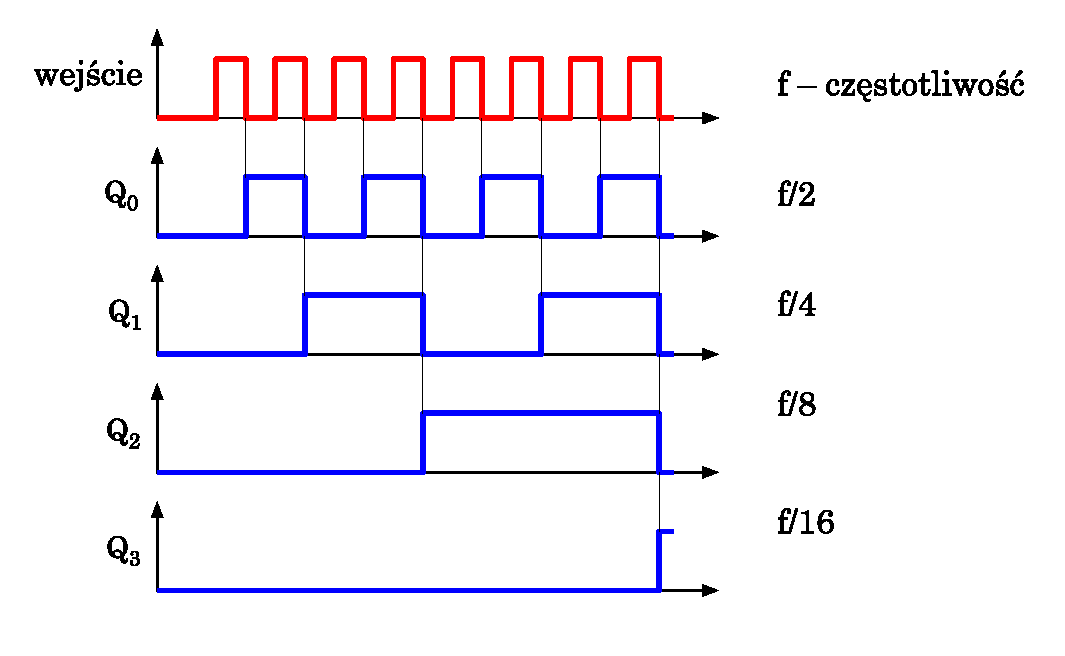
\includegraphics[scale=0.55]{grafiki/Licznik_freq.eps}
        \caption{Wizualizacja redukcji częstotliwości dla odpowiedniej ilości zastosowanych wejść,
        \\Źródło: Opracowanie własne}
        \label{fig1:freq}
      \end{figure}

      \subsubsection{jednobitowy Modulo 2}
        Licznik Modulo 2 przechodzi przez dwa stany (0 i 1). Zbudowany jest z jednego przerzutnika JK. Przy każdym zboczu narastającym sygnału zegarowego, przerzutnik JK zmienia swój stan z 0 na 1 lub z 1 na 0.
        
        \begin{figure}[!ht]
          \centering
          \includegraphics[scale=0.55]{grafiki/Licznik_JK_mod_2.eps}
          \caption{Schemat licznika jednobitowego modulo 2 zbudowanego z przerzutnika JK,
          \\Źródło: \href{https://spe.if.uj.edu.pl/literatura}{Strona wykładów}}
        \end{figure}

      \subsubsection{czterobitowy Modulo 16}
        Licznik Modulo 16 jest rozwiniętą wersją poprzedniego, składa się z 4 przerzutników JK co pozwala na przechodzenie przez 16 różnych stanów (od 0000 do 1111 w kodzie binarnym).
        \begin{figure}[!ht]
          \centering
          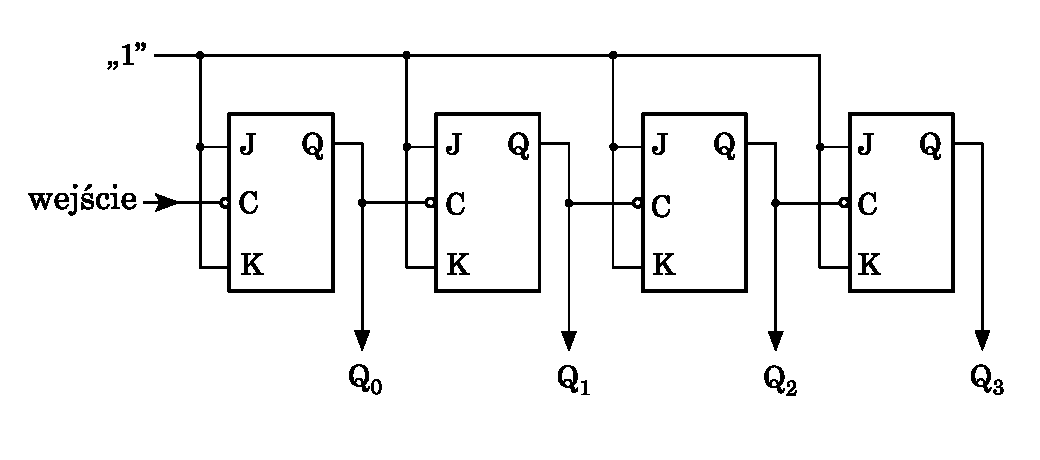
\includegraphics[scale=0.55]{grafiki/Licznik_JK_mod_16.eps}
          \caption{Schemat licznika czterobitowego modulo 16 zbudowanego z przerzutnika JK,
          \\Źródło: Opracowanie własne}
          \label{fig3:mod16}
        \end{figure}
        \pagebreak

      \subsubsection{czterobitowy Modulo 10}
        Tworzenie liczników o liczbie stanów różniej od potęgi dwójki jest bardziej skomplikowane. Realizuje się je przy pomocy dodatkowej bramki logicznej. W tym przypadku została użyta bramka NAND z wejściami $Q_1$ oraz $Q_3$ -- są to bity odpowiadające binarnej dziesiątce (1010). Wypuszczenie sygnału z tej bramki na wejścia \textit{Reset} przerzutników JK pozwala na ograniczenie zakresu licznika z 16 do 10.
        \begin{figure}[!ht]
          \centering
          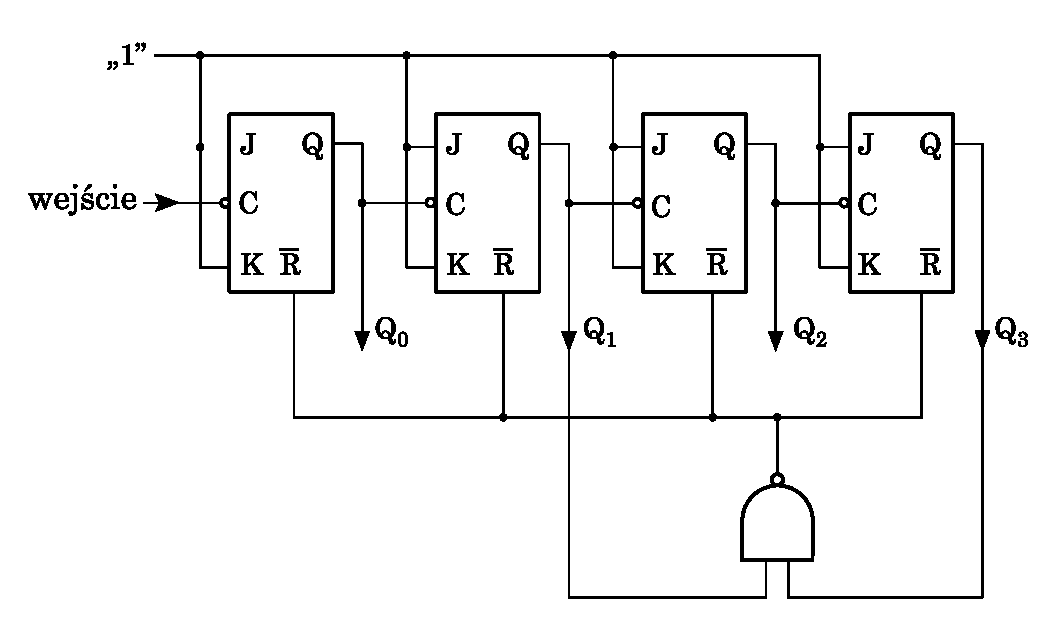
\includegraphics[scale=0.55]{grafiki/Licznik_JK_mod_10.eps}
          \caption{Schemat licznika czterobitowego modulo 10 zbudowanego z przerzutnika JK,
          \\Źródło: Opracowanie własne}
          \label{fig4:mod10}
        \end{figure}

  \section{Ćwiczenia}
        Przed rozpoczęciem ćwiczeń zostały sprawdzone wszystkie komponenty znajdujące się na płytce (impulsatory, wskaźniki, Próbnik, piny $5V$).
    \subsection{Ćwiczenie 5.1}
      \subsubsection{Własności wejść \textit{c}, \textit{d}}
        Pierwsze zadanie polegało na zbudowaniu synchronicznego przerzutnika RS. Zastosowane miały zostać układy scalone 7400 i 7410. Dwie z bramek miały posiadać po trzy wejścia. Wejścia dodatkowe $c$ i $d$ musiały zostać podłączone do $0V$ albo $5V$ poneważ bez tego układ nie zadziałałby.

        \begin{figure}[!ht]
          \centering
          \includegraphics[scale=0.55]{grafiki/RS_sync_zajecia.jpg}
          \caption{Schemat przerzutnika asynchronicznego RS typu latch zbudowany z układów 7400 i 7410 na zajęciach,
          \\Źródło: \href{https://spe.if.uj.edu.pl/literatura}{Strona wykładów}}
        \end{figure}
        \pagebreak
        
        Zwarcie wejść $c$ oraz $d$ z $5V$ zapewniło poprawne działanie układu. Wykorzystane do tego zostały dwa oporniki $1k\Omega$. Oporniki zostały dobrane według specyfikacji płytek dostępnej na stronie internetowej pracowni.


        Natomiast podłącznie wejść $c$ oraz $d$ do $0V$ (użyte zostały do tego oporniki $100\Omega$) zagwarantowało na obu przerzutnikach stały wysoki sygnał, co za tym idzie, wyjścia $Q$ oraz $\overline{Q}$ wskazywały równocześnie 1. Jest stan zakazany oznaczający niepoprawne działanie układu.

        \begin{figure}[!ht]
          \begin{minipage}{.5\textwidth}
            \centering
            \includegraphics[scale=0.06]{grafiki/RS_async_zdj_5V.png}
            \caption{Poprawnie zbudowany układ RS-latch z zegarem wpiętym na stałe do stanu wysokiego oraz wejściami $c$ i $d$ również zwartymi z $5V$. Wejścia $Q$ oraz $\overline{Q}$ wizualizowane są na dwóch wskaźnikach led,
            \\Źródło: Opracowanie własne}
          \end{minipage}
          \begin{minipage}{.5\textwidth}
            \centering
            \includegraphics[scale=0.05]{grafiki/RS_async_zdj_0V.png}
            \caption{Układ RS-latch z zegarem wpiętym na stałe do stanu wysokiego oraz wejściami $c$ i $d$ zwartymi z $0V$. Wejścia $Q$ oraz $\overline{Q}$ wizualizowane są na dwóch wskaźnikach led,
            \\Źródło: Opracowanie własne}
          \end{minipage}
        \end{figure}

      \subsubsection{Przebieg w czasowy}
        Drugą częścią zadania było podpięcie fali prostokątnej z generatora do powstałego układu oraz wizualizacja reakcji przerzutnika. Sygnał z generatora wchodził na wejście zegarowe. Jak jesteśmy w stanie zauważyć na poniższym rysunku, rekacja była widoczna tylko gdy zegar wskazywał stan wysoki.

        \begin{figure}[!ht]
          \centering
          \includegraphics[scale=0.35]{grafiki/5.1_CLK_Q.png}
          \caption{Zestawienie sygnału zegarowego (kanał 1) oraz wyjścia $\overline{Q}$ układu RS-latch (kanał 2) z zauważalnymi zmianami stanów w czasie stanu wysokiego zegara,
          \\Źródło: Opracowanie własne}
        \end{figure}

    \subsection{Ćwiczenie 5.2}
      Kolejne zadnie polegało na zbadaniu przerzutnika jednozboczowego D 
      znajdującego się na układzie scalonym 7474. Stan logiczny 1 podany został na wejścia $1CLR$ oraz $1PRE$ za pomocą górnego impulsatora($\overline{Q}$).

      \begin{figure}[!ht]
        \begin{minipage}{.5\textwidth}
            \centering
            \begin{tabular}{|c|c|c|c|c|c|}
              \hline
              \small \textbf{PR} & \small \textbf{CLR} & \small \textbf{CLK} & \small \textbf{D} & \small \textbf{Q} & \small $\mathbf{\overline{Q}}$ \\
              \hline
              L & H & X & X & H & L \\
              H & L & X & X & L & H \\
              \textcolor{red}{L} & \textcolor{red}{L} & \textcolor{red}{X} & \textcolor{red}{X} & \textcolor{red}{H} & \textcolor{red}{H} \\
              H & H & $\uparrow$ & H & H & L \\
              H & H & $\uparrow$ & L & L & H \\
              H & H & L & X & $Q_0$ & $\overline{Q_0}$ \\
              \hline
              \end{tabular}
              
            \caption{Tablica prawdy dla przerzutnika D,
            \\Źródło: \href{https://pdf1.alldatasheet.com/datasheet-pdf/view/50913/FAIRCHILD/7474.html}{Alldatasheet.com}}
        \end{minipage}
        \begin{minipage}{.5\textwidth}
          \centering
          \includegraphics[scale=0.35]{grafiki/7474_scheme.jpg}
          \caption{Schemat wejść/wyjść układu 7474,
          \\Źródło: \href{https://pdf1.alldatasheet.com/datasheet-pdf/view/50913/FAIRCHILD/7474.html}{Alldatasheet.com}}
        \end{minipage}
      \end{figure}

      Legenda tablicy prawdy: \\
      H -- wysoki stan logiczny \\
      X -- wysoki ulb niski stan logiczny \\
      L -- niski stan logiczny \\
      $\uparrow$ -- Rekacja na zboczne narastające \\
      $Q_0$ = Stan poprzedni układu \\
      \textcolor{red}{Kolor czerwony oznacza niestabilną konfigurację.}

      Sprawdzone zostały oba przerzutniki znajdujące się na płytce. Pominięty został stan gdy $PR = 0$ i $CLR = 0$ ponieważ jest on stanem zakazanym tego układu w którym wyjścia mogą zmieniać się w sposób nieoczekiwany.

      \begin{figure}[!ht]
        \begin{minipage}{.5\textwidth}
          \centering
          \includegraphics[scale=0.35]{grafiki/5.2_CLK_Q_D.png}
          \caption{Przebieg czasowy zegara oraz wyjścia $1Q$ układu 7474,
          \\Źródło: Opracowanie własne}
        \end{minipage}
        \begin{minipage}{.5\textwidth}
          \centering
          \includegraphics[scale=0.1]{grafiki/Przerzutnik_D_zdj.png}
          \caption{Poprawnie podłączony przerzutnik D z wejściami $1CLR$ oraz $1PRE$ wpiętymi do logicznej 1 za pomocą górnego impulsatora,
          \\Źródło: Opracowanie własne}
        \end{minipage}
      \end{figure}
      \pagebreak
  
    \subsection{Ćwiczenie 5.3}
      Poniższa część zajęć polegała na zbadaniu płytki 7475 wybierając jeden z czterech przerzutników D “latch” wyzwalanych poziomem.


      \begin{figure}[!ht]
        \centering
        \includegraphics[scale=0.45]{grafiki/7475.png}
        \caption{Schemat wejść/wyjść układu 7475,
        \\Źródło: \href{https://eduinf.waw.pl/inf/prg/010_uc/7475.php}{7475 -- cztery przerzutniki D Latch}}
      \end{figure}

      Sprawdzony został przerzutnik znajdujący się najbardziej z lewej przy wyżłobieniu. Nie wykazał on żadnych nieprawidłowości w działaniu. Poniżej załączam jeden z poprawnych przebiegów czasowych dla tego układu. Jak jesteśmy wstanie zauważyć, układ aktualizuje stan wyjściowy na bieżąco tylko wtedy gdy sygnał zegarowy jest wysoki.

      \begin{figure}[!ht]
        \begin{minipage}{.5\textwidth}
          \centering
          \includegraphics[scale=0.35]{grafiki/5.3_CLK_Q_D_latch.png}
          \caption{Przebieg czasowy zegara oraz wyjścia $1Q$ układu 7475,
          \\Źródło: Opracowanie własne}
        \end{minipage}
        \begin{minipage}{.5\textwidth}
          \centering
          \includegraphics[scale=0.1]{grafiki/Przerzutnik_D_latch_zdj.png}
          \caption{Poprawnie podłączony przerzutnik D-latch. Wejście D zostało wpięte do impulsatora,
          \\Źródło: Opracowanie własne}
        \end{minipage}
      \end{figure}

    \subsection{Ćwiczenie 5.4}
      Jest to zadanie które wymagało użycia przerzutników JK do zbudowania licznika jednobitowego modulo 2. Wykorzystany do tego został układ 7493. Jedną z cech liczników jest to, że mogą zostać użyte jako dzielniki częstotliwości[\ref{fig1:freq}].

      \begin{figure}[!ht]
        \begin{minipage}{.5\textwidth}
          \centering
          \includegraphics[scale=0.5]{grafiki/7493_01.png}
          \caption{Wewnętrzna sieć logiczna licznika 7493,
          \\Źródło: \href{https://eduinf.waw.pl/inf/prg/010_uc/7493.php}{7493 – 4-bitowy licznik dwójkowy (moduły 2 i 8)}}
        \end{minipage}
        \begin{minipage}{.5\textwidth}
          \centering
          \includegraphics[scale=0.5]{grafiki/7493_03.png}
          \caption{Oznaczenie wejść/wyjść w układzie 7493,
          \\Źródło: \href{https://eduinf.waw.pl/inf/prg/010_uc/7493.php}{7493 – 4-bitowy licznik dwójkowy (moduły 2 i 8)}}
        \end{minipage}
      \end{figure}

      Jak jesteśmy wstanie zauważyć na poniższym zrzucie ekranu z osylospku, uzyskana częstotliwość jest faktycznie dwukrotnie mniejsza. Na wejściu podany został $1Hz$ a otrzymana wartość wskazuje $500mHz$.

      \begin{figure}[!ht]
        \begin{minipage}{.5\textwidth}
          \centering
          \includegraphics[scale=0.4]{grafiki/5.4_mod_2_freq.png}
          \caption{Przebieg czasowy częstotliwości wejściowej oraz efektu uzyskanego z układu redukującego,
          \\Źródło: Opracowanie własne}
        \end{minipage}
        \begin{minipage}{.5\textwidth}
          \centering
          \includegraphics[scale=0.1]{grafiki/7493_mod_2.png}
          \caption{Zbudowany na zajęciach układ dzielący częstotliwość przez 2,
          \\Źródło: Opracowanie własne}
        \end{minipage}
      \end{figure}

    \subsection{Ćwiczenie 5.5}
      Kolejne zadanie wymagało użycia tego samego układu 7493. Celem było zwiększenie możliwości licznika do wykonywania akcji modulo 16. Został on wykonany według schematu(\ref{fig3:mod16}).

      \begin{figure}[!ht]
        \centering
        \includegraphics[scale=0.1]{grafiki/7493_mod_16.png}
        \caption{Zbudowany na zajęciach licznik modulo 16,
        \\Źródło: Opracowanie własne}
      \end{figure}

      W celu wizualizacji poprawnego działania układu wyjścia $Q_0$ -- $Q_3$ zostały podłączone do wskaźników led. Wideo z poprawnego działania układu dostępne jest pod tym linkiem\href{https://youtu.be/uBRxpVXEhjw}{[LINK]}.

    \subsection{Ćwiczenie 5.6}
    
      Ostatnie zadanie wymagajace układu 7493 polegało na zbudowaniu modulo 10. Został on wykonany według schematu(\ref{fig4:mod10}). Jest to nic innego jak układ mod 16 ograniczony bramką NAND gdy "doliczymy"\mbox{} do dziesięciu. jest ona wbudowana w układ 7493 co ułatwiło montaż licznika.

      \begin{figure}[!ht]
        \centering
        \includegraphics[scale=0.07]{grafiki/7493_mod_10.png}
        \caption{Zbudowany na zajęciach licznik modulo 10 z wykorzystaniem bramki NAND,
        \\Źródło: Opracowanie własne}
      \end{figure}
      \pagebreak

      Jak i w poprzednim zadaniu wizualizacja działania układu wyjścia została pokazana na wskaźnikach led. Wideo z poprawnego działania układu dostępne jest pod tym linkiem\href{https://www.youtube.com/watch?v=QPkW2fbpPyo}{[LINK]}.

  \section{Omówienie wyników}
    \subsection{Ćwiczenie 5.1}
      Na początku, pierwszą rzeczą do wykonania było zbadanie roli wejść $c$ oraz $d$. Z obserwacji dokonanych podczas zajęć wynika, że wpięcie jednego z tych wejść do logicznego zera, powoduje, że wyjście(odpowiadające danej bramce) nie jest w stanie zmienić swojego stanu(natura bramki NAND). Można by powiedzieć, że wejścia te służą do wyłączania z użytku jednego z wyjść $Q$, $\overline{Q}$ lub obu naraz -- wskazują one wtedy stan wysoki.

      Samo działanie układu odbyło się zgodnie z oczekiwaniami i nie wskazywało na błędne jego podłączenie.

    \subsection{Ćwiczenie 5.2}
      W drugim zadaniu również nie dostrzeżono żadnych problemów po wykonaniu układu. Zamiast impulsatora jako sygnału zegarowego został użyty generator, a do wyświelania wyjścia oscyloskop. Wejścia $PR$ oraz $CLR$ służą odpowiednio w układzie jako $Set$ oraz $Reset$. Niski poziom logiczny na wejściu $PR$ lub $CLR$ powoduje odpowiednio ustawienie na 1 lub wyzerowanie wyjścia $Q$ przerzutnika.
      
    \subsection{Ćwiczenie 5.3}
      Jak widać po przebiegu czasowym wyświelanym na oscyloskopie, układ został zbudowany poprawnie. Odpowiadał on tylko na wejście $D$ gdy zegar był w stanie wysokim.
    \subsection{Ćwiczenie 5.4}
      Screenshot sygnału zegarowego oraz wyjścia układu pięknie ilustruje nam zmianę w częstotliwości sygnału -- jest ona dwukrotnie mniejsza. Oprócz tego zauważalny jest spadek w amplitudzie co może wynikać ze zniekształceń sygnału lub niewłaściwie dopasowanej impedancji.
    \subsection{Ćwiczenie 5.5}
      Nagranie wideo ilustruje poprawne działanie układu.
    \subsection{Ćwiczenie 5.6}
      Nagranie wideo dokumentuje poprawne zatrzymanie się licznika na liczbie binarnej odpowiadającej dziesiątce.
  \section{Podsumowanie}
    W trakcie laboratorium wykonano różne układy z przerzutników JK i D, w tym przerzutnik RS, synchroniczny przerzutnik D oraz liczniki modulo. Każdy z układów został zbudowany zgodnie z teoretycznymi założeniami i przetestowany za pomocą generatora fali prostokątnej oraz diod LED. W rezultacie, wszystkie układy działały poprawnie i zgodnie z oczekiwaniami, co potwierdzają uzyskane przebiegi czasowe.
  \section{Notatki z zajęć}

    \begin{figure}[!ht]
      \begin{minipage}{.5\textwidth}
        \centering
        \includegraphics[scale=0.2]{grafiki/notatki1.png}
        \caption{Notatki wykonane w czasie zajęć,
        \\Źródło: Opracowanie własne}
      \end{minipage}
      \begin{minipage}{.5\textwidth}
        \centering
        \includegraphics[scale=0.05]{grafiki/notatki2.png}
        \caption{Zdjęcie pomocnicze wykonane w czasie zajęć,
        \\Źródło: Opracowanie własne}
      \end{minipage}
    \end{figure}

    \begin{figure}[!ht]
      \centering
      \includegraphics[scale=0.05]{grafiki/notatki3.png}
      \caption{Zdjęcie pomocnicze wykonane w czasie zajęć,
      \\Źródło: Opracowanie własne}
    \end{figure}

\end{document}